\section*{Implementation}
\begin{figure}[width=\textwidth]
    \begin{centering}
        \vspace{-.8cm}
        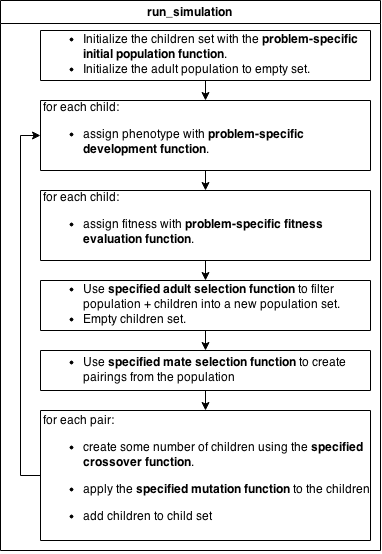
\includegraphics[width=0.9\linewidth]{img/EA-loop.png}
        \caption{Implementation outline}
        \label{evo-loop}
    \end{centering}
\end{figure}

Python 3.4 was used to implement this project.
For plotting results I used the library \textit{matplotlib}.

%The evolutionary loop is located in the \texttt{run\_simulation} function that takes a key-value object with all the parameters required to run a simulation.
I tried to stay close to the EA flow as illustrated in Figure 1 in the EA appendices\cite{ea-appendices}.
%Figure \ref{evo-loop} shows the loop implementation.

Problems are Python modules that contain functions for generating initial populations,
development of phenotypes from genotypes, and fitness evaluation.

The problem independent functions are defined as standalone functions that get all the information they need via parameters.

%All the development functions I have implemented are simple one to one transformations from string to list format.
%The evolutionary loop itself is not aware of the formats,
%so as long as there is consistency between the problem and the crossover and mutation functions,
%any kind of geno- or phenotype format and complex development function should be supported.

%The fitness functions I made all return values in the 0 to 1 range,
%but the algorithm works for any range of fitness values.

Since the project emphasises modularity,
I tried to use generic functional programming as much as possible.

The evolutionary loop function requires a configuration object to run,
which specifies all the details of the simulation,
including the problem module itself,
numeric parameters,
and the various other functions.
If new functions are defined they can be loaded into a configuration with a simple import statement.

\begin{minipage}{\linewidth}
    \begin{lstlisting}[language=Python, caption=Creating a new problem type.]
NAME = 'IS_EMPTY_STRING'

def generate_initial_population(population_size, genome_size):
    return tuple(random_string(len=genome_size) for _ in range(population_size))

def geno_to_pheno(genotype):
    return genotype.split()

def fitness_evaluation(pheno):
    if len(pheno) == 0:
        return 1.0
    else:
        return 0.0
    \end{lstlisting}
\end{minipage}


\begin{minipage}{\linewidth}
    \begin{lstlisting}[language=Python, caption=Plugging in a different mate selection function.]
config.update({
   'mate_selection_method': some_function_reference,
   'mate_selection_args': {
        'parameter_a': 10,
        'parameter_b': "Foo"
    }
})
    \end{lstlisting}
\end{minipage}

%If the problem requires any special parameters (like the z in LOLZ) this can be specified in the \texttt{problem\_parameters} sub-object, which will be passed to the functions as keyword arguments.

Specifics such as the formats of geno- and phenotypes or fitness values are not the concern of the loop itself,
only the functions that are plugged in.

The simplest user interface for the program is to use a text editor to create a configuration in a \texttt{.py}-file and call the \texttt{run\_simulation} function with it.
Another option is implemented in \texttt{main.py}:
a command line interface that allows the user to choose a preset,
then modify the parameters before running the simulation.

\section*{One-Max problem}
\begin{figure}[width=\textwidth]
    \begin{centering}
        \vspace{-1cm}
        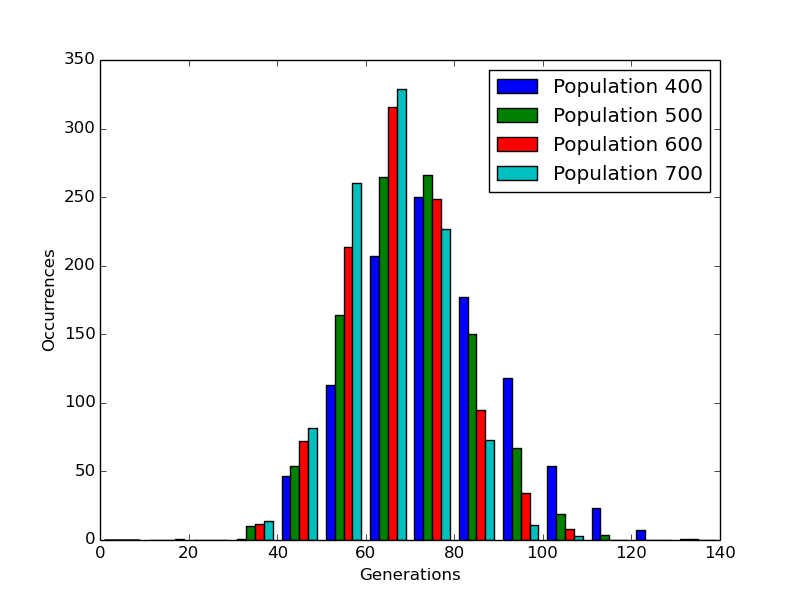
\includegraphics[width=\linewidth]{img/3x1000.png}
        \caption{Generation number where an optimal solution is found. 4x1000 trials.}
        \label{different_population_sizes}
    \end{centering}
\end{figure}

To find a minimal population size I created configurations that differed only by population size,
ran them 1000 times each,
and plotted the generation numbers where an optimal solution was found in a histogram.
%This histogram can be seen in Figure \ref{different_population_sizes}.
Using this I visually identified 600 as a suitable value.
At that size there were only a few ($1.3\%$) outliers that exceeded 100 generations.

\begin{figure}[width=\textwidth]
    \begin{centering}
        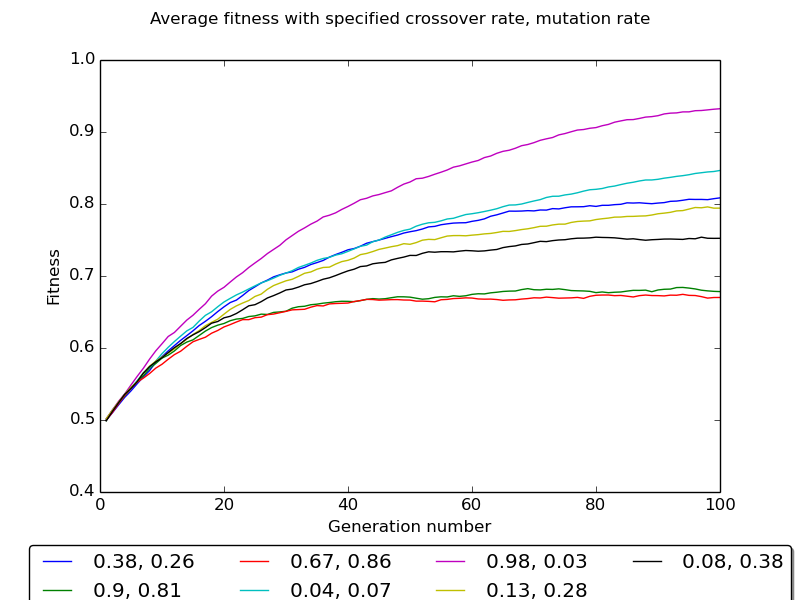
\includegraphics[width=\linewidth]{img/random_rates.png}
        \caption{Averaged graph for 10 runs of each configuration}
        \label{different_rates}
    \end{centering}
\end{figure}

\subsection*{Different rates}
To figure out the crossover and mutation rates I started out by generating random values,
running simulations with those values 10 times in a row and averaging the lines for each configuration.
The plot of this can be seen in Figue \ref{different_rates}.

%The crossover scheme used was the "mix" one where for each position in the new genome one bit was selected from a random parent.
%For mutation I used the "per genome" scheme.

From the results it can be seen that it is not beneficial to have a high mutation rate.
It is clear that it is the crossover that is supposed to steer the population in the right direction,
the mutation is just there to shake things up a little bit.

Based on this I decided to proceed with a high crossover rate of $0.90$ and a very low mutation rate of $0.01$ per genome.

\subsection*{Parent selection}
\begin{figure}[width=\textwidth]
    \begin{centering}
        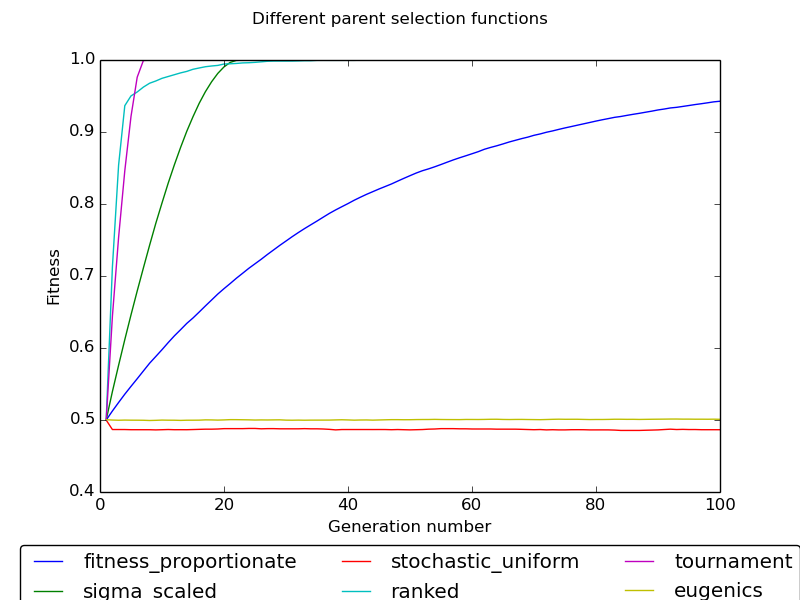
\includegraphics[width=\linewidth]{img/different_parent_selection_100N.png}
        \caption{Testing different parent selection functions.}
        \label{different_function}
    \end{centering}
\end{figure}

When testing different parent selection methods I again averaged multiple trials for each type.
As Figure \ref{different_function} shows,
the stochastic uniform and "eugenics" methods failed to produce better individuals.
The fitness proportionate method worked fine but slowly, and by 100 generations was getting close to an optimal solution.
But three functions performed significantly better.
The ranked roulette method got off to the best start but struggled to find the last $5\%$ for an optimal solution.
The tournament method is the best in this test,
it found an optimal solution within 10 generations.
The sigma scaled method worked simillar to the tournament, but at a slower rate.

\subsection*{Different target}
Modifying the target string means modifying the fitness evaluation function to correctly evaluate the candidate vs. the target string.
As long as this is done correctly, nothing about the difficulty will change.
The recombination and mutation function will not at all be affected by this change.

I tested this statement by creating two configurations that differed only by target string and averaged the plots for 100 trials of each.
The results was two practically identical lines (figure \ref{different_targets}).

\begin{figure}[width=\textwidth]
    \begin{centering}
        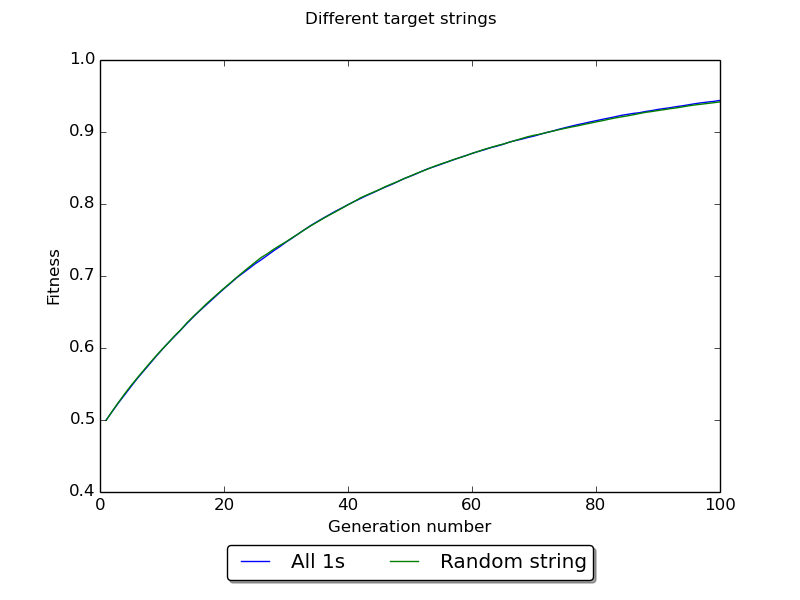
\includegraphics[width=\linewidth]{img/different_targets.png}
        \caption{100 averaged trials of searching for all 1s, and searching for a random string. The lines are practically identical.}
        \label{different_targets}
    \end{centering}
\end{figure}

\subsection*{Changing the problem}
\begin{figure}[width=\textwidth]
    \begin{centering}
        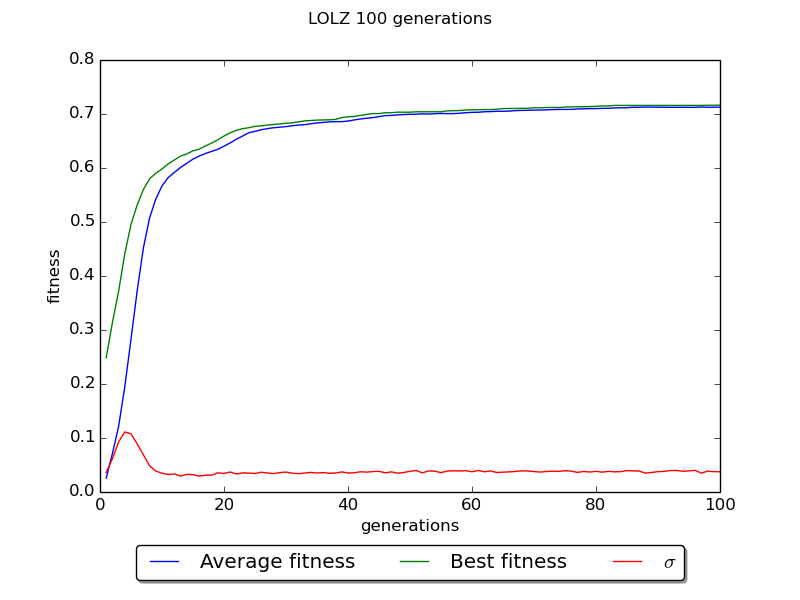
\includegraphics[width=\linewidth]{img/lolz_100x100.png}
        \caption{Average 100 trials of LOLZ z=21}
        \label{lolz_100x100}
    \end{centering}
\end{figure}

When running the same configuration for the LOLZ problem,
the average of multiple trials flattens out somewere between $0.5$ and $1.0$ (figure \ref{lolz_100x100}).
This is because in some trials,
the population moves in the direction of the local maximum of 21 zeroes.
If this happens the population gets stuck at a max fitness level of $21/40 = 0.525$.
In other trials the population starts heading towards the global maximum and reaches average fitness of $1.0$.
Since there is a 50/50 chance of the population going for leading ones or leading zeroes,
the average eventually line positions itself between $1.0$ and $0.525$.

\section*{Surprising Sequences}
\begin{figure}[width=\textwidth]
    \begin{centering}
        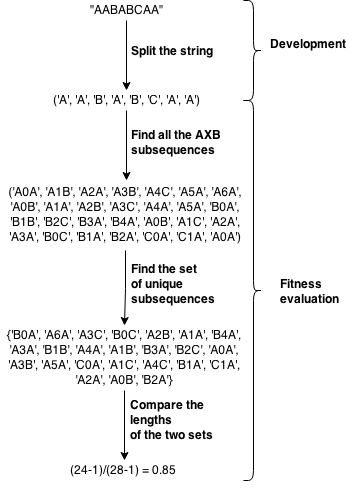
\includegraphics[width=\linewidth]{img/surprising_process.png}
        \caption{Example of how a genotype is processed.}
        \label{}
    \end{centering}
\end{figure}

Working with the type system in Python shaped the formats of geno- and phenotypes in my implementation greatly.
%Since Python has no explicit type for bits it would be very cumbersome to try to force my types into some faux bit format.
I went with more high level representation of the types than perhaps intended.
In the case of the Surprising Sequences problem the genotypes are regular Python strings composed of the characters in the character set of size S.
Phenotypes are just the list version of the same string.

I considered doing more operations during the development function,
specifically finding the $AX_nB$ substrings at that point,
but ultimately felt it was more appropriate to let that be the job of the fitness function.

The fitness function scans through each phenotype to find all the subsequences of the format $AX_nB$.
For finding globally surprising sequences it will find the subsequences for any $n$, for locally surprising sequences it will stop after $n=0$.
It then compares the number of \textit{unique} $AX_nB$ subsequences to the total number of subsequences.

\begin{align*}
    f
    =
    \frac{
        \left|\text{unique $AX_nB$ }\right| - 1
    }{
        \left|\text{total $AX_nB$}\right| - 1
    }
    &~&
    \text{for} ~ L > 2
\end{align*}

This will give a score of $1.0$ if the sequence is completely surprising.
For locally surprising sequences it will score $0.0$ if the sequence is just the same character repeated,
while that sequence will get a low but non-zero score when evaluated for globally surprisingness.

\begin{table}[h!]
    \begin{tabular}{lllll}
        S  & Population & Generations & L%   & Sequence
        \\        \hline
        3  & 50              & 1           & 10
        %  & C, B, B, A, A, B, C, A, C, C
        \\
        5  & 50              & 383         & 26
        %& C, E, A, A, E, D, C, A, D, A, B, B, A, C, B, D, D, B, C, D, E, B, E, E, C, C
        \\
        10 & 50              & 876         & 94
        %& G, E, H, J, C, G, A, C, C, E, C, H, A, E, E, I, J, G, I, B, E, J, J, F, D, E, B, C, D, G, G, C, A, F, A, D, J, I, I, F, B, A, A, H, C, F, G, H, I, E, G, B, I, G, D, B, B, F, J, A, J, E, A, I, A, G, J, H, G, F, E, F, C, B, J, B, D, H, D, F, F, H, F, I, D, C, I, H, B, H, H, E, D, D
        \\
        15 & 50              & 620         & 196
        %& E, A, F, F, H, H, C, C, D, F, E, J, K, C, L, M, K, E, O, N, I, D, D, H, G, H, B, I, E, I, I, J, D, K, A, K, D, O, C, M, O, F, B, O, E, E, M, L, E, G, K, N, N, M, N, C, N, A, O, B, A, D, G, A, C, O, H, M, D, A, I, G, J, C, E, L, H, O, I, O, K, J, F, D, B, H, K, O, L, N, J, I, B, G, F, K, L, F, J, O, D, J, N, O, A, B, E, K, G, M, J, J, B, M, I, K, I, N, K, H, I, L, L, G, C, I, M, E, H, E, N, D, L, B, D, E, D, N, F, N, G, G, O, G, L, O, J, M, C, B, J, H, A, A, E, B, L, D, C, G, N, B, C, F, A, J, A, N, L, A, H, N, H, D, I, F, O, M, F, I, A, M, B, F, M, H, F, C, K, K, F, G, B, K, M, A
        \\
        20 & 200             & 548        & 343
        %& F, M, F, O, F, A, F, E, R, I, A, P, P, B, A, J, T, S, N, E, B, Q, G, L, K, T, H, M, E, J, F, P, S, D, A, G, N, P, C, D, J, K, L, R, R, O, N, B, G, I, L, P, O, P, G, G, P, K, F, L, N, G, T, B, J, C, F, T, G, H, F, R, M, B, B, C, B, R, K, M, N, Q, J, N, R, J, I, P, H, N, S, F, I, B, T, K, H, O, A, Q, M, A, C, R, H, G, Q, E, K, J, E, T, D, N, O, D, R, D, O, K, K, B, S, E, A, H, E, P, T, A, K, D, B, F, H, K, C, J, R, C, O, J, J, S, J, H, I, N, L, E, Q, P, A, N, D, E, H, B, E, C, N, H, J, Q, B, M, R, T, O, B, O, M, H, A, R, S, T, P, D, F, F, Q, L, T, Q, I, J, M, L, F, D, D, G, A, M, S, S, K, P, N, A, L, H, H, Q, T, T, R, E, I, T, N, J, G, O, I, O, G, C, S, A, E, E, N, M, G, E, O, Q, N, K, R, G, M, K, O, C, E, D, M, O, S, M, T, J, D, T, L, O, L, I, I, S, O, T, E, L, L, J, B, D, I, G, F, K, S, I, F, B, N, F, S, R, B, I, H, L, S, P, R, L, C, P, I, M, Q, S, L, D, P, Q, C, C, L, G, D, K, G, K, A, D, S, B, H, C, Q, H, S, G, R, A, I, K, I, E, M, D, C, T, F, J, P, J, A, T, I, Q, F, N, T, M, M, C, M, I, D, H, P, E, G, S, H, R
        \\
    \end{tabular}
    \caption{Longest L found in less than 1000 generations, local surprising}
\end{table}
\begin{table}
    \begin{tabular}{lllll}
        S  & Population & Generations & L%  & Sequence
        \\ \hline
        3  & 200 & 1    & 7
        %& B, C, A, C, C, B, A
        \\
        5  & 200 & 6    & 12
        %& D, C, A, D, B, C, B, E, A, A, C, D
        \\
        10 & 200 & 748  & 24
        %& E, D, A, B, C, E, I, J, G, B, J, H, G, F, C, F, A, D, D, I, E, B, H, C
        \\
        15 & 200 & 176  & 36
        %& L, K, L, G, O, I, B, G, F, J, C, B, I, H, E, D, A, O, M, J, K, N, A, K, D, C, M, B, O, O, H, F, I, G, L, N
        \\
        20 & 200 & 81   & 46
        %& I, B, G, N, P, P, Q, S, G, L, N, C, O, M, T, B, H, L, F, I, R, K, J, T, E, A, C, A, B, L, A, S, H, J, E, O, Q, D, M, K, P, I, M, N, F, G
        \\
    \end{tabular}
    \caption{Longest L found in less than 1000 generations, global surprising}
\end{table}

\section*{Difficulty}
One-Max is the easiest.
In the solution space there are no local maximas,
every increment leads towards the single global maximum.
Combining two fit parents is likely to produce a child that is also very fit.

LOLZ is more difficult than One-Max because the z parameter means there exists a local maximum.
If the population starts trending towards that maximum it is unlikely that they will ever find the global maximum,
as the sub-population with leading zeroes will outcompete and eradicate the subpopulation with leading ones.

Another issue is that combining two parents with simillar fitnesses is not guaranteed to produce a fit individual at all, since the two parents might be fit in different ways.
There is also the fact that an individual like "0111111" has the potential to be the parent of a very fit individual,
but is itself very unfit and therefore might not get to mate at all.
These are not problems that occur in One-Max.

The two Suprising Sequences problems are the most difficult,
with globally suprising being even more difficult than locally surprising,
since a globally surprising sequence must satisfy the criteria for local surprisingness and then some.

Unlike the previous problems where the fitness topology has only one global maxima (and one local maxima in LOLZ) there are many global and local maxima for the surprising sequences.
Finding the correct path to a global maximum is not easy,
and most trials become "needle in a haystack"-situations.
It is also more difficult to tell if a random mutation is beneficial or not,
since each genome component factors into the fitness in so many ways.

\section*{References}
[1] Anonymous. EA Appendices, January 2014
